\section{Computing}

The LHCb experiment provides an extremely challenging software environment. Requirements for such a software project include management of both large amounts of data as well as high rates of data; managing software written by a large number of collaborating scientists; managing frequent improvements and changes in algorithms; the ability to provide a common interface between generated data and measured data such that meaningful comparisons can be made; a constantly changing detector environment and the encapsulation of data relevant to a wide range of users.

The LHCb software is based on the Gaudi software architecture and framework \cite{Antunes-Nobrega:835156}. This framework is specifically design for use in the field of high energy physics and based on the concept of object orientated programming. Well defined interfaces are defined between components of the framework so that each component can be modified in a self contained manner without affecting other components. A schematic view of the Gaudi architecture is shown in figure \ref{fig: state of gaudi appliaction}, describing a typical state of the software model. 

\begin{figure}[h]
	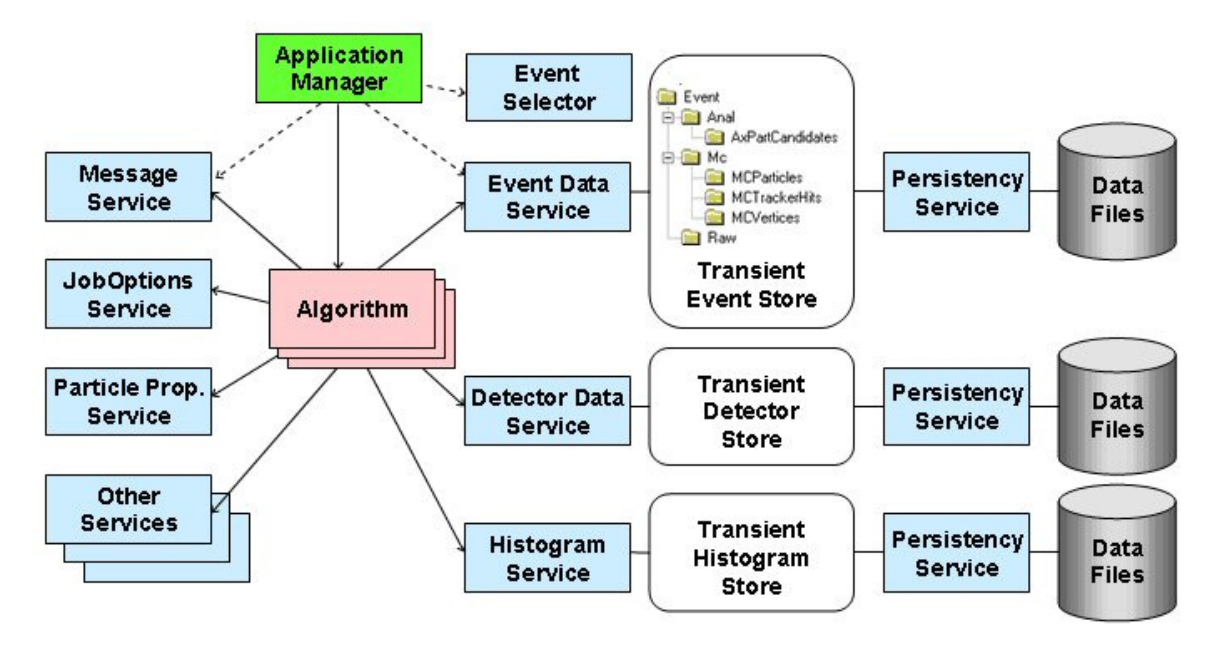
\includegraphics[width=\columnwidth]{/Users/admin/Dropbox/PhD/Thesis/Chapters/detector/computing/images/GaudiArchitecture.png}
	\caption{A state diagram of a typical application build on the Gaudi framework}
	\label{fig: state of gaudi appliaction}
\end{figure}

Unique to Gaudi architecture in comparison to other object orientated frameworks is the distinction between data and algorithms. In the Gaudi architecture algorithms themselves are objects and act on data objects (e.g. A track fitting algorithm acts on detector hit objects to form a track rather than the hits themselves forming a track). The motivation of this approach is shown in the persistency of algorithms and data objects. Algorithms are methods typically used to create objects such as tracks from detector hits; these methods are constantly being improved over the lifetime of the experiment. In contrast to this the models describing data are more stable (e.g. the concept of a track is not expected to change). Making a distinction between the algorithm and data decouples the two enabling the ability to modify the algorithms without affecting the data.

Each phase of the data processing is encapsulated into an application built on the Gaudi framework. Monte Carlo event generation and detector response to the generated particles is handled by the Gauss application, the output of this phase is in the form of detector hits and is used as input for the Boole application. The Boole application applies a detector response to the hits generated by the Gauss application digitising the hits into a format which mimics measured data. Additional hits are added from from Spillover events and LHC background and the digitisation step of the readout electronics, as well as of the L0 trigger hardware are simulated. The next phase of data processing is to reconstruct objects from the digitised hits, this is achieved through the Brunel application. Since the output from Boole is designed such that it models the detector output the algorithms used by Brunel are exactly the same for both generated data and data produced from measured collisions, decoupling the reconstruction phase completely from the generation phase. The output from the reconstruction phase is then proceeded by an analysis phase, the application for this phase is the DaVinci application. This phase is focused on the application of more sophisticated algorithms acting on high level objects such as particles and secondary vertices. This includes the reconstruction of exclusive decay channels and high level background correction. The overall application and data flow is outlined in figure \ref{fig: application data flow}.

\begin{figure}[h]
	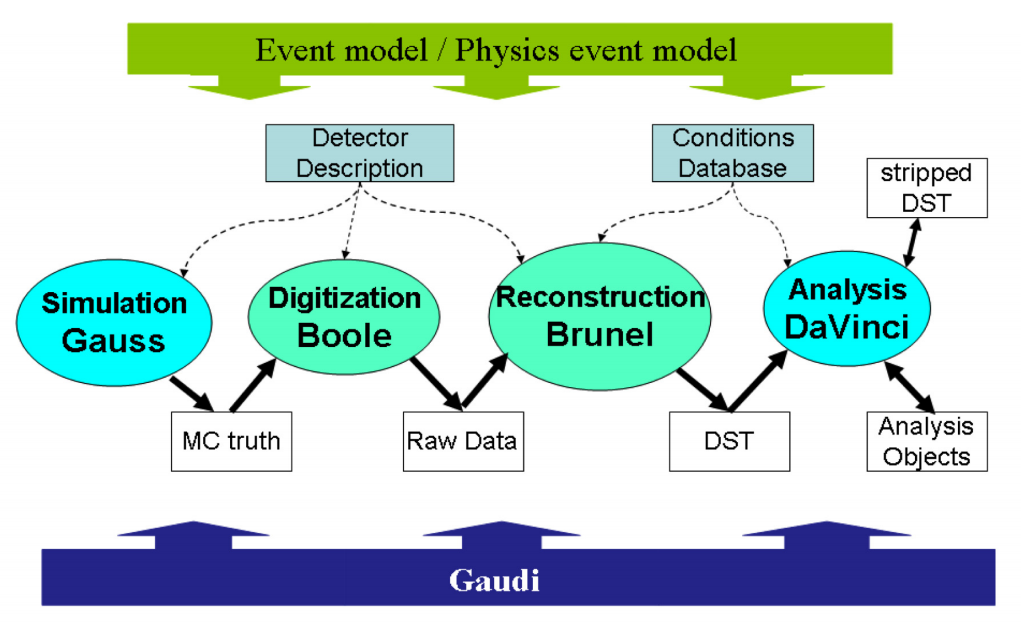
\includegraphics[width=\columnwidth]{/Users/admin/Dropbox/PhD/Thesis/Chapters/detector/computing/images/application_data_flow.png}
	\caption{A schematic of application processes and data flow. Underlying all the applications is the Gaudi framework. The arrows represent the transfer of input and output data.}
	\label{fig: application data flow}
\end{figure}

%In addition to the applications stated above there are many more applications focused on aspects of the operation of the LHCb detector e.g. online monitoring, interactive analysis and visualisation applications. For further information see \ref{}.

Information about the state of the LHCb detector at a given time is accessed via the Conditions Database service. This information includes such things as the temperature and pressure in certain detector elements as well as the alignment parameters used to describe the detector. The values stored in the database are dependent on several variables such as the time, version and data source of the data; each combination of variables is identified by a unique tag. Similarly information about the structure and materials of the detector elements are accessed via the Detector Descriptions Database and accessed via the Detector Description Service.

%The LHCb software is structured into several projects, each with a well defined functionality or application. Each project comprises of a set of packages. A package is defined as a set of files which together provide a well defined functionality. For example the Rec project contains packages related to the reconstruction process; these packages are organised such that they pertain to certain aspects of the reconstruction such as the tracking, calorimeters and particle identification. Dependencies between projects enable packages to be shared across projects, when building the software the dependencies are managed by the Configuration Management Tool (CMT).

To make use of the grid computing service the LHCb software uses the Distributed Infrastructure with Remote Agent's Control project (DIRAC). This together with the job submission application named Ganga, enables users to perform large scale physics analysis without having to the need for a complete understanding of the computing challenges behind their physics analyses.

